\chapter{Calcul littéral --\\ Distributivité}\label{ChDistributivite}

\vspace{5cm}
\begin{acquis}
\begin{itemize}
\item Connaître et utiliser la distributivité.
\item Savoir traiter le cas particulier du signe $-$ devant une parenthèse.
\columnbreak
\item Savoir résoudre des problèmes en utilisant la distributivité.
\end{itemize}
\end{acquis}


\activites  
\begin{activite}[Les rectangles]
\ImageDroite{%
\begin{enumerate}
    \item Sur ton cahier, reproduis les rectangles roses de telle sorte qu'ils forment un grand rectangle. Pourquoi peut-on les regrouper facilement ?
    \item Calcule l'aire totale des rectangles roses de deux façons différentes. (L'une d'elles ne doit comporter qu'une seule multiplication.)
    \item Reprends les deux questions précédentes pour les rectangles verts.
    \item Wilfrid affirme qu'il peut calculer la somme des aires des six rectangles en utilisant une seule multiplication. Comment fait-il ? Pourquoi est-ce possible ?
\end{enumerate}
}{\vspace*{2cm}
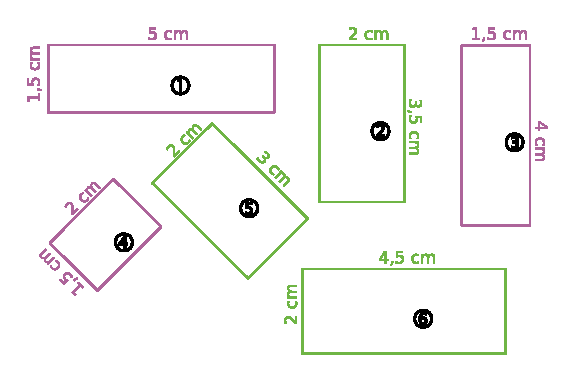
\includegraphics[width=.45\linewidth]{DiA01}}
\end{activite}
 




\begin{activite}[Avec des mots]
En lisant son cours de mathématiques sur le chapitre \og Distributivité \fg, Odile remarque qu'il existe des phénomènes très similaires dans certaines phrases.

\vspace{1em}\textbf{1\up{ère} Partie}\vspace{1em}

Odile se dit qu'on peut parfois développer le sujet ou le verbe d'une phrase. 
Par exemple : Dans la phrase \og Marius et Gaëlle mangent. \fg, on peut développer le verbe, ce qui donne : \og Marius mange et Gaëlle mange. \fg.

\begin{enumerate}
\item Développe les phrases suivantes :
\og Audrey relit et apprend ses leçons. \fg ;
\og La pluie, le vent et le froid l'empêchaient de sortir de la maison. \fg.
\item Invente une phrase de ton choix dans laquelle on peut développer le verbe.

\vspace{1em}\textbf{2\up{e} Partie}\vspace{1em}

Odile se dit qu'on peut aussi utiliser des mots mathématiques dans ces phrases.

\item Développe la phrase suivante : \og 78 et 12 sont multipliés par 5. \fg.
\end{enumerate}
\end{activite}
 







\begin{activite}[Calcul réfléchi]
Lucie connaît ses tables de multiplication jusqu'à 10 et voudrait construire la table de 11. Anthony, son voisin, lui explique que c'est facile de la trouver et lui donne un exemple à l'oral : 
\og onze fois quatorze \fg, c’est \og dix fois quatorze plus une fois quatorze \fg.
Comme Lucie n'a pas très bien compris, Anthony écrit alors :
\begin{align*}
    11 \times 14 	&= 10 \times 14 + 1 \times 14 \\
		&= 140 + 14 \\
		&= 154 \\
\end{align*}

\begin{enumerate}
    \item Écris la phrase puis le calcul pour $11 \times 15$ et $17 \times 11$.
    \item Recopie puis complète la table de 11 suivante.

\renewcommand*\tabularxcolumn[1]{>{\centering\arraybackslash}m{#1}}
\begin{lctableau}{\linewidth}{12}
\hline
$\times$ & 10 & 11 & 12 & 13 & 14 & 15 & 16 & 17 & 18 & 19 & 20 \\ \hline
11 & & & & & 154 & & & & & & \\ \hline
\end{lctableau}

    \item\label{DisAc01} Lucie propose alors de calculer $13 \times 21$ en procédant de façon similaire. Elle note ses calculs intermédiaires dans le tableau ci-dessous.

\begin{center}
\begin{minipage}[c]{.35\linewidth}
\renewcommand*\tabularxcolumn[1]{>{\centering\arraybackslash}m{#1}}
\begin{lctableau}{\linewidth}{3}
\hline
$\times$ & 20 & 1  \\ \hline
13 & 260 & 13\\ \hline
\end{lctableau}
\end{minipage}
\end{center}

Elle obtient : $13 \times 21 = 273$.

Explique comment elle a obtenu 273 comme résultat.

    \item Calcule les produits suivants en présentant les résultats intermédiaires dans un tableau.
        \subitem $12 \times 34$
        \subitem $17 \times 1 001$
    \item Anthony fait remarquer que l'on peut aussi calculer facilement $13 \times 19$ à partir des résultats intermédiaires notés dans le tableau. Calcule ce produit.
    \item Avec les tableaux que tu as construits à la question \ref{DisAc01}, quels autres produits peux-tu calculer facilement ? Écris-les puis calcule-les.
\end{enumerate}
\end{activite}





\begin{activite}[Développer $(a + b)(c + d)$]
\begin{enumerate}
    \item On considère le produit $P = 86 \times 53$. Justifie les égalités suivantes : $P = 86 \times 50 + 86 \times 3$ puis $P = 80 \times 50 + 6 \times 50 + 80 \times 3 + 6 \times 3$.

Déduis-en l'égalité : $(80 + 6) \times (50 + 3) = 80 \times 50 + 6 \times 50 + 80 \times 3 + 6 \times 3$ puis calcule $P$ sans poser de multiplication (et sans calculatrice !).
    \item Complète : $(a + b)(c + d) = ... \times (c + d) + ... \times (c + d) = ... + ... + ... + ...$.
    
Quelle propriété as-tu utilisée ? Combien de fois ? En quoi a été transformé le produit initial ?
    \item \subitem a) Complète : $(3x  - 2)(5x + 4) = (... + ...) \times (... + ...)$.
    \subitem b) Déduis-en le développement de ce produit.
    \subitem c) Procède de même avec le produit $(2  - y)(2y  - 5)$.
    \item Pour développer le produit $(2a + 3)(3a  - 4)$, on peut poser la multiplication comme indiqué ci-dessous.
    
    \begin{center}
        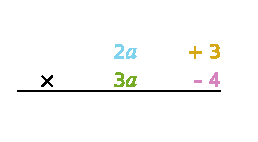
\includegraphics[width=.33\linewidth]{DiA02}
    \end{center}
    
    Effectue-la sans oublier le décalage.
\end{enumerate}
\end{activite}


\cours
\section{Développer une expression littérale}

\subsection{La distributivité simple}

\begin{propriete}
Soient $k$, $a$ et $b$ trois nombres relatifs. Pour \MotDefinition{développer une expression}{}, on distribue un facteur à tous les termes entre parenthèses :

\begin{align*}
    \boldsymbol{k \times} (a + b) &= \boldsymbol{k \times} a + \boldsymbol{k \times} b\\
    \boldsymbol{k \times} (a - b) &= \boldsymbol{k \times} a - \boldsymbol{k \times} b\\
\end{align*}

%\begin{center}
%    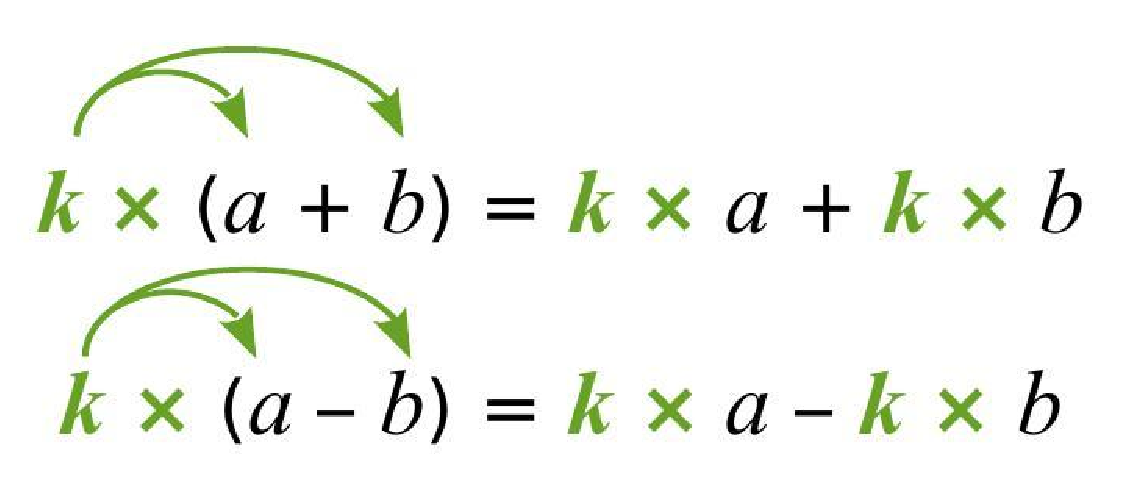
\includegraphics[width=.35\linewidth]{DiC01}
%\end{center}
\end{propriete} 


\begin{exemple*1}

Développe l'expression suivante : $C = - 3,5(x - 2)$.

\correction

\begin{tabular}{lcl}
$C = \boldsymbol{- 3,5 \times} (x - 2)$ & $\longrightarrow$ & On replace le signe $\boldsymbol{\times}$ dans l'expression. \\
$C = \boldsymbol{(- 3,5)} \times x + \boldsymbol{(- 3,5)} \times (- 2)$ & $\longrightarrow$ & On distribue le facteur $-3,5$ aux termes $x$ et $-2$. \\
$C = - 3,5x + 7$ & $\longrightarrow$ & On calcule et on simplifie l'expression. \\
\end{tabular}
\end{exemple*1}




\subsection{Cas particulier : \MotDefinition{distribuer un signe $-$}{}}

\begin{propriete}
Lorsqu'une parenthèse est précédée d'une signe $-$, c'est comme si toute la parenthèse était multipliée par $-1$. Le moins se distribue donc comme un nombre, en utilisant la règle du produit des signes :
\begin{align*}
    \boldsymbol{-1 \times} (a + b) &= \boldsymbol{-1 \times} a + \boldsymbol{( -1 ) \times} b = - a + (-b) = - a - b \\
    \boldsymbol{-1 \times} (a - b) &= \boldsymbol{-1 \times} a - \boldsymbol{( -1 ) \times} b = - a - (-b) = - a + b \\
\end{align*}

%\begin{center}
%    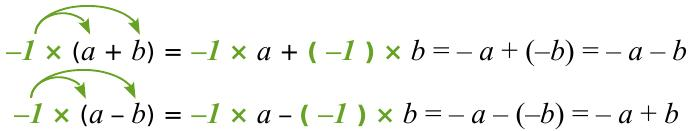
\includegraphics[width=.65\linewidth]{DiC02}
%\end{center}
\end{propriete}

\begin{exemple*1}

Développe l'expression suivante : $A = - (x - 2) + (- 2x + 3) - (-1 - 2x)$.

\correction

\begin{tabular}{lcl}
$A = - (x - 2) + (- 2x + 3) - (-1 - 2x)$ & & \\
$A =  - x + 2 + (- 2x + 3) +1 + 2x$ & $\longrightarrow$ & On distribue le signe $-$ de la 1\up{ère} et de la 3\up{e} parenthèse. \\
$A = - x + 2 - 2x + 3 +1 + 2x$ & $\longrightarrow$ & On peut enlever la parenthèse précédée d'un $+$. \\
$A = - 3x + 6$ & $\longrightarrow$ & On calcule et on simplifie l'expression. \\
\end{tabular}
\end{exemple*1}





\subsection{La \MotDefinition{double distributivité}{}}


\begin{propriete}
Pour tous nombres relatifs $a$, $b$, $c$ et $d$ :

\begin{minipage}[c]{.6\linewidth}
    \centering
    $(\boldsymbol{a} + \boldsymbol{b})(c + d) = \boldsymbol{a}c + \boldsymbol{a}d + \boldsymbol{b}c + \boldsymbol{b}d$
    %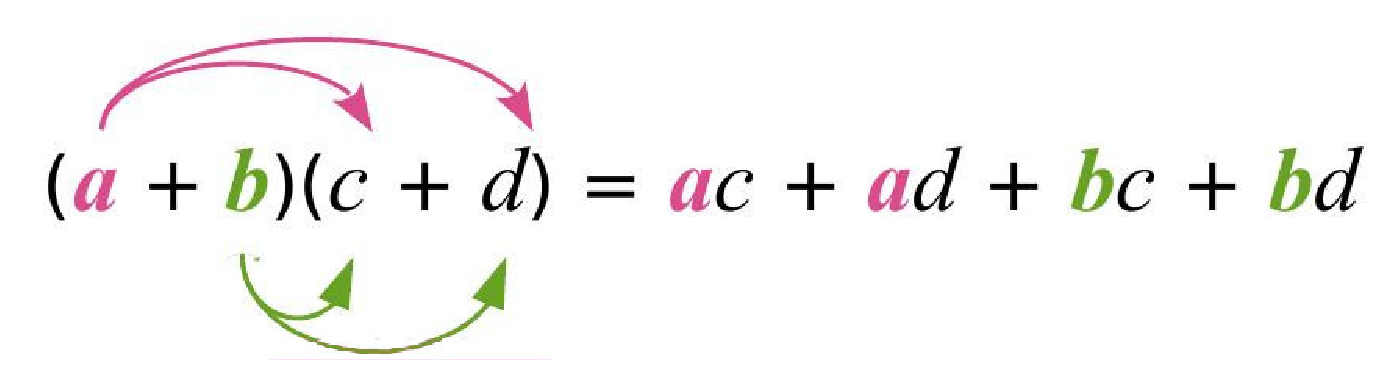
\includegraphics[width=\linewidth]{DiC03}
\end{minipage}%
\hfill%
\begin{minipage}[c]{.38\linewidth}
    \centering
    
\includegraphics[width=.7\linewidth]{DiC04}
\end{minipage}
\end{propriete} 

\begin{exemple*1}

Développe et simplifie l'expression suivante : $D = (3x + 1)(y - 4)$.

\correction

\begin{tabular}{lcl}
$D = (3x + 1)(y + (- 4))$ & $\longrightarrow$ & On transforme la soustraction. \\
$D = \boldsymbol{3x \times} y + \boldsymbol{3x \times} (- 4) + \boldsymbol{1 \times} y + \boldsymbol{1 \times} (- 4)$ & $\longrightarrow$ & On applique la double distributivité. \\
$D = 3xy - 12x + y - 4$ & $\longrightarrow$ & On calcule les produits et on simplifie. \\
\end{tabular}
\end{exemple*1}







\exercicesbase
\begin{colonne*exercice}
\serie{Développer}


\begin{exercice}[]
Développe puis réduis les expressions :
\begin{colenumerate}{2}
\item $A = 3 \times (x + 2)$
\item $B = 7 \times (x - 6)$
\item $C = 1 \times (x + 5)$
\item $D = 4 \times (5 - x)$
\item $E = 1,6(x - 0,5)$
\item $F = 4(x + 1)$
\item $G = 7(3x - 8)$
\item $H = 6(2x + 9)$
\end{colenumerate}
\end{exercice}

\begin{exercice}[]
Développe puis réduis les expressions :
\begin{colenumerate}{2}
\item $A = x(x + 2)$
\item $B = x(x - 6)$
\item $C = 3x(x + 5)$
\item $D = 5x(x - 1)$
\item $E = 6x(2 + 9x)$
\item $F = x(x^2 - 4)$
\end{colenumerate}
\end{exercice}

\begin{exercice}[]
Développe les expressions suivantes :
\begin{colenumerate}{2}
\item $A = 3(x + 6)$
\item $B = 5(6 -y)$
\item $C = -7(2z -3)$
\item $D = -8(-5 -3y)$
\item $E = 6(4x -9)$
\item $F = -12(-5 + 3z)$
\end{colenumerate}
\end{exercice}

\begin{exercice}[]
Développe les expressions suivantes :
\begin{colenumerate}{2}
\item $A = (-3 + y) \times 9$
\item $B = -6(2x -7)$
\item $C = (3t + 2) \times 8$
\item $D = -8(9 -7x)$
\item $E = -8z(4 -3z)$
\item $F = 3y(-4 + 6y)$
\end{colenumerate}
\end{exercice}

\begin{exercice}[]
Développe les expressions suivantes :
\begin{colenumerate}{2}
\item $A = x(x + 4)$
\item $B = 7y(2 - 9y)$
\item $C = -2y(5 -y)$
\item $D = (9 -3t) \times 4t$
\end{colenumerate}
\end{exercice}

\begin{exercice}[]
Développe et réduis les expressions :
\begin{colenumerate}{2}
\item $A = 11 + 2(x -6)$
\item $B = -3(2y -4) -2y$
\item $C = 7 -4(8 -2a) + a$
\item $D = -15 -9(-5 + 3b)$
\item $E = -5(6 -3z) -9 + z$
\item $F = 12x -4(6 -3x)$
\end{colenumerate}
\end{exercice}

\begin{exercice}[]
Développe et réduis les expressions :
\begin{colenumerate}{1}
\item $A = 3x -5 + 5(2x -2)$
\item $B = 4y -6(3 -2y) + 4(y -1)$
\item $C = 5t^2 + 3(2t -3) -2t(t -5)$
\end{colenumerate}
\end{exercice}



\serie{Double distributivité}





\begin{exercice}[]
Développe et réduis les expressions :
\begin{colenumerate}{2}
\item $A = (x + 4)(x + 3)$
\item $B = (y + 3)(2y + 8)$
\item $C = (3z + 4)(5 -6z)$
\item $D = (-7t + 8)(3 -5t)$
\end{colenumerate}
\end{exercice}

\begin{exercice}[]
Développe et réduis les expressions :
\begin{colenumerate}{2}
\item $A = (7 -3x)(9x -3)$
\item $B = (-2 -3y)(4 -8y)$
\item $C = (4a + 6)(-3 -5a)$
\item $D = (5z -7)(8z + 2)$
\end{colenumerate}
\end{exercice}

\begin{exercice}[]
Développe et réduis les expressions :
\begin{colenumerate}{2}
\item $A = (a + 1)^2$
\item $B = (5x + 2)^2$
\item $C = (3y -4)^2$
\item $D = (4 -x)^2$
\end{colenumerate}
\end{exercice}

\begin{exercice}[]
Développe et réduis les expressions :
\begin{colenumerate}{2}
\item $A = 3(x + 1)(x -5)$
\item $B = 2(-3 -t)(t -7)$
\item $C = -(y + 5)(3y -6)$
\item $D = x(2x -5)(2 -x)$
\end{colenumerate}
\end{exercice}

\begin{exercice}[]
On considère les expressions :

\[A = (x + 2)(x -3) + (x -3) \quad \text{et} \quad B = (2x -3)^2 \]

\begin{colenumerate}{1} 
\item Développer et réduire les deux expressions.
\item Calculer $A$ pour $x = 3$.
\item Calculer $B$ pour $x = 1,5$.
\end{colenumerate} 
 
\end{exercice}

\begin{exercice}[]
On considère le rectangle ci-dessous. Exprime en fonction de $x$ :

\begin{center}
    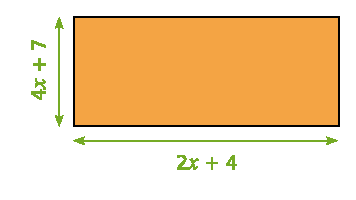
\includegraphics[width=.7\linewidth]{DiEe01}
\end{center}

\begin{colenumerate}{1} 
\item son périmètre sous la forme d'une expression réduite ;
\item son aire sous la forme d'une expression factorisée ;
\item son aire sous la forme d'une expression développée et réduite.
\end{colenumerate} 
 
\end{exercice}

\begin{exercice}[]
Parmi les expressions suivantes, retrouve celles qui sont égales et justifie ta réponse :
\begin{colenumerate}{2}
\item $A = 16 -4x2$
\item $B = (4 -2x)^2$
\item $C = (4 -2x)(4 + 2x)$
\item $D = 4x2 -16x + 16$
\end{colenumerate}
\end{exercice}

\end{colonne*exercice}


\exercicesappr
\begin{colonne*exercice}
\begin{exercice}[Par paires]
Regroupe par deux les expressions qui sont égales.
\begin{colenumerate}{2}
\item $A = 6x^2 + 4$
\item $B = 6x^2 + 2$
\item $C = 3x^2(2x + 4)$
\item $D = 3(2x^2 + 1) - 1$
\item $E = 6x(x^2 + 2x)$
\item $F = 8x^2 - 4 - 2x^2 + 8$
\end{colenumerate}
\end{exercice}

\begin{exercice}[Une expression en trop]
Trouve l'intrus.
\begin{colenumerate}{2}
\item $A = 4(2x - 3)$
\item $B = 8x - 12$
\item $C = 5(x - 4) + 3x + 8$
\item $D = 10(x - 1) - 2x$
\item $E = 6(2x - 3) + 2(3 - 2x)$
\end{colenumerate}
\end{exercice}

\begin{exercice}[Substitution]
Soit $G = 3(4x - 2)$. Calcule $G$ lorsque :

\begin{colenumerate}{2} 
\item $x = 5$
\item $4x - 2 = 7$
\item $12x = 11$
\item $6x = 5$
\item $2x - 1 = 3$
\item $3x = 25$
\end{colenumerate} 
\end{exercice}

\begin{exercice}[]
\textsl{Marie dit qu'en ajoutant deux nombres impairs, on obtient toujours un nombre impair.}

\begin{colenumerate}{1} 
\item Prouve-lui qu'elle a tort à l'aide d'un contre-exemple.
\item \ref{DisEA01} En utilisant la variable $n$, écris une expression désignant un nombre pair puis une autre désignant un nombre impair.
\item Utilise la question \label{DisEA01} pour démontrer à Marie que la somme de deux nombres impairs n'est jamais impaire.
\end{colenumerate} 
\end{exercice}

\begin{exercice}[Au zoo]
Au zoo, il y a des cacatoès et des koalas. On peut y dénombrer 50 têtes et 140 pattes.

\begin{colenumerate}{1} 
\item Si besoin, recherche, dans un dictionnaire ou sur internet, le nombre de pattes d'un cacatoès et d'un koala.
\item On note $c$ le nombre de cacatoès. Exprime le nombre de koalas en fonction de $c$.
\item Écris une expression $P$ représentant le nombre de pattes en fonction de $c$.
\item Développe puis réduis $P$.
\item Calcule le nombre de cacatoès puis le nombre de koalas.
\end{colenumerate} 
\end{exercice}

\begin{exercice}[Un carré qui grandit]
Soit ABCD un carré de 5\,cm de côté. 

\begin{colenumerate}{1} 
\item Calcule le périmètre $\mathcal{P}_1$ et l'aire $\mathcal{A}_1$ de $ABCD$.
\item On augmente ses côtés de $k$\,cm. 

Exprime, en fonction de $k$ :
        \subitem la longueur $L$ du nouveau côté ;
        \subitem le nouveau périmètre $\mathcal{P}_2$ de ce carré ;
        \subitem la nouvelle aire $\mathcal{A}_2$ de ce carré ;
        \subitem l'augmentation du périmètre ;
        \subitem l'augmentation de l'aire.
\end{colenumerate}
\end{exercice}




\begin{exercice}[La pyramide de Gelo]
Godtfred a construit une pyramide de briques Gelo. Il y a une brique au premier niveau, 4 briques au deuxième niveau, 9 briques au troisième niveau, comme sur le schéma suivant.

\begin{center}

\includegraphics[width=.5\linewidth]{DiEa01}
\end{center}

\begin{colenumerate}{1} 
\item \label{DisEA02} Combien y a-t-il de briques au quatrième niveau ? Au 20\up{e} niveau ? Au $n$\up{e} niveau ?
\item Combien y a-t-il de briques au total lorsque la pyramide compte un niveau ? Deux niveaux ? Trois niveaux ? Quatre niveaux ?

Godtfred veut savoir combien de briques seront nécessaires pour construire une pyramide à vingt niveaux. Ne voulant pas faire un gros calcul, il cherche sur internet une formule lui donnant le résultat. Il a trouvé les trois expressions suivantes où $n$ représente le nombre de niveaux :
\begin{align*}
    A &= - 6n + 7 \\
    B &= \dfrac{5n^2 - 7n +4}{2} \\
    C &= \dfrac{n(n+1)(2n+1)}{6} \\
\end{align*}

Godtfred veut alors vérifier la véracité de ces informations.
\item En testant chacune des formules par les valeurs trouvées à la question \ref{DisEA02}, quelles sont les formules que l'on peut éliminer d'office ?
\item Godtfred demande à son professeur si la formule non éliminée est exacte. Il lui répond par l'affirmative. Combien de briques sont nécessaires pour construire la pyramide à vingt niveaux ?
\end{colenumerate} 
\end{exercice}

\begin{exercice}[Tracé d'un U dans une feuille]
En cours d'Arts Plastiques, le professeur a distribué aux élèves des feuilles carrées de 15\,cm de côté.

Il leur demande de découper un rectangle de largeur 5\,cm pour former la lettre U. 

\begin{colenumerate}{1} 
\item Marine découpe un rectangle de longueur 8\,cm (et de largeur 5\,cm).

Calcule le périmètre du U de Marine.

    \begin{center}
    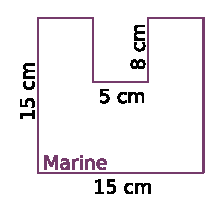
\includegraphics[width=.5\linewidth]{DiEa02}
    \end{center}
 
\item Ses amies Alison et Laura ont découpé des rectangles de largeur 5\,cm mais de longueurs différentes : celui d'Alison a une longueur de 6,3\,cm alors que celui de Laura a une longueur de 9,6\,cm. 
 
Calcule les périmètres des U d'Alison et de Laura. Quelle partie du calcul est la même pour tous les U ?

\item Après tous ces calculs, Kévin remarque que si $L$ désigne la longueur du rectangle en centimètres et $\mathcal{P}$ le périmètre du U en centimètres, alors  $\mathcal{P}= 60 + 2L$. Calcule $\mathcal{P}$ lorsque $L = 7,5$\,cm puis lorsque $L = 10$\,cm.
\item Priscilla dit : \og On peut encore simplifier : $60 + 2 = 62$ donc $\mathcal{P} = 62 L$. \fg. Utilise l'expression proposée par Priscilla pour calculer $\mathcal{P}$ lorsque $L = 10$\,cm. Qu'en déduis-tu ?
\end{colenumerate} 
\end{exercice}

\begin{exercice}[Distributivité à gogo]

\begin{colenumerate}{1} 
\item On veut développer l'expression $A = 2(5x + 2)(3x + 1)$. Pour cela, développe d'abord l'expression $2(5x + 2)$ puis termine le développement de $A$.
\item Développe le produit $(x + 2)(3x + 2)$ et déduis-en le développement de :
    \subitem $B = (x + 2)(3x + 2)(x + 4)$
\item En t'inspirant des questions précédentes, développe les expressions suivantes :
    \subitem $C = 4(5x -1)(3x + 3) $
    \subitem $D = (1 -x)(1 + x)(2x + 1)$
\end{colenumerate}
\end{exercice}




\begin{exercice}[Idée fausse]

\begin{colenumerate}{1} 
\item On considère les expressions $A = (2x + 3)^2$ et $B = (2x)^2 + 32$. Calcule ces expressions pour $x = 0$ et pour $x = 10$. Qu'en déduis-tu ?
\item Peut-on dire que pour tout nombre $a$ et tout nombre $b$ non nuls, les expressions $(a + b)^2$ et  $a^2 + b^2$ sont égales ? Justifie. Développe alors l'expression $(a + b)^2$.
\item On considère les deux expressions $C = (2x + 3) (2x -3)$ et $D = (2x)^2 -3^2$. Calcule ces expressions pour $x = 0$ puis pour $x = 10$. Qu'en déduis-tu ? Démontre-le.
\item Développe alors l'expression : $(a + b)(a -b)$.
\end{colenumerate} 
\end{exercice}



\begin{exercice}[Calcul mystère]

\begin{colenumerate}{1} 
\item \label{DisEA03} Calcule les expressions $2001 \times 1999 -2000^2$ et $47 \times 45 -46^2$. Que remarques-tu ?
\item Développe et réduis l'expression suivante :
\[(x + 1)(x -1) -x^2\]
\item Les résultats obtenus à la question \ref{DisEA03} étaient-ils prévisibles ? Justifie.
\item Écris d'autres expressions du même style et donne leurs résultats sans poser d'opération.
\end{colenumerate} 
\end{exercice}




\begin{exercice}[Petites démonstrations]

\begin{colenumerate}{1} 
\item Que dire de la somme de deux nombres pairs ? De deux nombres impairs ? Pourquoi ?
\item La somme de deux nombres consécutifs est‑elle paire ou impaire ? Justifie.
\item Que dire du produit de deux nombres pairs ? De deux nombres impairs ? De deux nombres consécutifs ? Pourquoi ?
\end{colenumerate} 
\end{exercice}



\serie{Problèmes}



\begin{exercice}[]
On considère les deux parallélépipèdes rectangles suivants :
    
    \begin{center}
    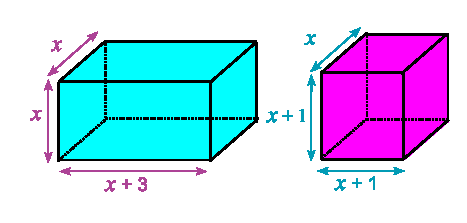
\includegraphics[width=.9\linewidth]{DiEa03}
    \end{center}

\begin{colenumerate}{1} 
\item \label{DisEA05} Calcule les deux volumes pour $x = 1$.

Que remarques-tu ?
\item Exprime, en fonction de $x$, les deux volumes. Que remarques-tu ? Comment expliquer alors le résultat de la question \ref{DisEA05} ?
\end{colenumerate} 
\end{exercice}




\begin{exercice}[]
On considère la figure suivante ($x$ désigne un nombre supérieur ou égal à 2) : 

    \begin{center}
    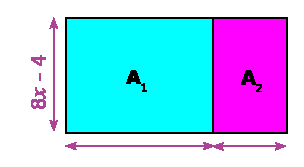
\includegraphics[width=.7\linewidth]{DiEa04}
    \end{center}

\begin{colenumerate}{1} 
\item Exprime en fonction de $x$ les aires $\mathcal{A}_1$ et $\mathcal{A}_2$.
\item Déduis-en une expression de l'aire totale $\mathcal{A}$ de la figure.
\item Calcule $\mathcal{A}_1$, $\mathcal{A}_2$ et $\mathcal{A}$ pour $x = 6$.
\end{colenumerate} 
\end{exercice}




\begin{exercice}[]
Isabelle achète $t$ kilogrammes d'oignons à 3,20\,€ le kilo et elle achète le double en masse de tomates à 2,30\,€ le kilo. Exprime, en fonction de $t$, le montant de ses achats en euros.
\end{exercice}



\begin{exercice}[]
Adeline achète 5 CD et 3 DVD. On notera $x$ le prix en euros d'un CD. Un DVD coûte 10 euros de plus qu'un CD.

\begin{colenumerate}{1} 
\item \label{DisEA06} Écris, en fonction de $x$, la dépense d'Adeline en euros. Développe et réduis l'expression trouvée.
\item En utilisant l'expression obtenue au \ref{DisEA06}, calcule, en euros, la dépense d'Adeline si un CD coûte 15\,€.
\end{colenumerate} 
 
\end{exercice}

\begin{exercice}[] 
La figure ci-dessous représente un carré de 6\,cm de côté. $M$ est un point de $[AD]$ et $N$ est un point de $[AB]$ tels que : 

$AM = AN = x$ ($x$ est un nombre strictement positif).

    \begin{center}
    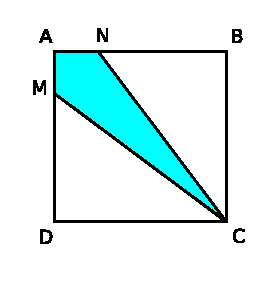
\includegraphics[width=.6\linewidth]{DiEa05}
    \end{center}

\begin{colenumerate}{1} 
\item Calculer, en fonction de $x$, les aires des triangles $MDC$ et $NBC$.
\item Calculer, en fonction de $x$, l'aire du quadrilatère $AMCN$.
\item Calculer ces trois aires pour $x = 2$\,cm. 
\end{colenumerate} 
\end{exercice}




\begin{exercice}[]
Une salle de concert peut contenir 600 places. Il y a $x$ places assises et les autres sont debout. Les places debout coûtent 15\,€ et les places assises 25\,€.

\begin{colenumerate}{1} 
\item Que représentent les expressions suivantes : $600 -x$ ; $25x$ et $15(600 -x)$ ?
\item Exprime, en fonction de $x$, la recette totale en euros si toutes les places sont prises.
\item Calcule cette recette si $x = 200$.
\end{colenumerate}
\end{exercice}

\end{colonne*exercice}

\connaissances
\QCMautoevaluation{Pour chaque question, plusieurs réponses sont proposées. Déterminer celles qui sont correctes.}

\begin{QCM}
\begin{GroupeQCM}

\begin{exercice}
Pour $x = -2$, $3x +5$ vaut...
\begin{ChoixQCM}{4}
\item $-1$
\item $11$
\item $-11$
\item $6$
\end{ChoixQCM}

\begin{corrige}
\reponseQCM{a}
\end{corrige}
\end{exercice}












\begin{exercice}
Lorsqu'on substitue $-3$ à $x$ dans $x^2 -5x$, on obtient...
\begin{ChoixQCM}{4}
\item $-3^2 -5 -3$
\item $(-3)^2 -5 \times (-3)$
\item $x^2 -5 \times (-3)$
\item $-3^2 -5 \times -3$
\end{ChoixQCM}

\begin{corrige}
\reponseQCM{a}
\end{corrige}
\end{exercice}


\begin{exercice}
La forme réduite de $15 -4x -5 + 2x$ est...
\begin{ChoixQCM}{4}
\item $10-6x$
\item $-2x+10$
\item $8x$
\item $-2x-20$
\end{ChoixQCM}

\begin{corrige}
\reponseQCM{a}
\end{corrige}
\end{exercice}



\begin{exercice}
La forme réduite de $(3x -6) - (-3x + 8)$ est...
\begin{ChoixQCM}{4}
\item $2$
\item $6x + 2$
\item $6x -14$
\item $6x^2 -14$
\end{ChoixQCM}

\begin{corrige}
\reponseQCM{a}
\end{corrige}
\end{exercice}


\begin{exercice}
La forme réduite de $(-b + 5) - (8 -6b)$ est...

\begin{ChoixQCM}{4}
\item $5b -3$
\item $-7b$
\item $-7b -3$
\item $-4b -3$
\end{ChoixQCM}

\begin{corrige}
\reponseQCM{a}
\end{corrige}
\end{exercice}


\begin{exercice}
La forme développée de $(5x -2)(2x -3)$ est...
\begin{ChoixQCM}{4}
\item $10x^2 -12x -6$
\item $10x -15x -4x -6$
\item $10x^2 -19x + 6$
\item $10x^2 -11x + 6 $
\end{ChoixQCM}

\begin{corrige}
\reponseQCM{a}
\end{corrige}
\end{exercice}


\begin{exercice}
\og Choisir un nombre x, faire la somme de son quotient par 3 et de 2 et multiplier le tout par 5 \fg.
\begin{ChoixQCM}{4}
\item $x + \dfrac{3}{2} \times 5$
\item $\dfrac{x}{3} + 2 \times 5$
\item $\dfrac{5(x+2)}{3}$
\item $5\left(\dfrac{x}{3}+2\right)$
\end{ChoixQCM}

\begin{corrige}
\reponseQCM{a}
\end{corrige}
\end{exercice}

\end{GroupeQCM}
\end{QCM}



\TravauxPratiques
\begin{TP}[Des phrases et des expressions littérales]

\vspace{1em}\textbf{1\up{ère} Partie : Programmes de calculs}\vspace{1em}


\item Voici un programme de calculs :

\begin{center}
    \begin{minipage}{.6\linewidth}
        \begin{oldalgorithme}
Choisir un nombre ;
Lui ajouter 1 ;
Multiplier le résultat par 3 ;  
Ajouter 4 au résultat.%
        \end{oldalgorithme}
    \end{minipage}
\end{center}

\vspace{.5em}

Appliquez ce programme au nombre 2.

\item Omar a appliqué ce programme pour un certain nombre et a trouvé 28. Laura dit alors que, pour retrouver le nombre de départ, il suffit de \og remonter \fg le programme de calculs en partant de la fin. Expliquez ce que veut dire Laura. Combien trouve-t-elle ?
\item \label{DisFC01} Voici un autre programme de calculs :


\begin{center}
    \begin{minipage}{.6\linewidth}
        \begin{oldalgorithme}
Choisir un nombre ;
Lui ajouter 3 ;
Multiplier le résultat par 2 ;
Ajouter le nombre du départ ;
Enlever 6 au résultat.%
        \end{oldalgorithme}
    \end{minipage}
\end{center}

\vspace{.5em}


Appliquez ce programme au nombre 5.

\item La méthode de Laura fonctionne-t-elle encore ? Pourquoi ?
\item Marc a trouvé une méthode pour trouver directement le nombre de départ, connaissant le résultat de la fin du programme. Expliquez cette méthode.
\item Construisez quatre programmes différents (dont au moins deux comme le programme de la question \ref{DisFC01}) qui transforment un nombre en un nombre quatre fois plus grand. 


 
\vspace{1em}\textbf{2\up{e} Partie : En français dans le texte}\vspace{1em}


Avant l'invention de l'algèbre, les mathématiciens utilisaient le langage courant pour écrire certaines propriétés, on pouvait énoncer la règle suivante :
\og Soit un nombre entier. Si on ajoute le nombre qui le précède et le nombre qui le suit, on obtient le double du nombre \fg.
\item En appelant $n$ le nombre, écrivez une égalité qui traduit cette phrase.
\item Procédez de la même façon pour le texte suivant : \og La différence des carrés de deux nombres entiers consécutifs est égale au double du plus petit augmenté de 1. \fg.
\item Développez et réduisez : $(x - 1)(x + 1)$ Chaque membre du groupe écrit en français un texte décrivant l'égalité obtenue.
\item Comparez vos textes. Écrivez ensemble celui qui vous paraît le plus clair.

\end{TP}




\newpage

\begin{TP}[Le Mistigri des expressions littérales]

   
\vspace{1em}\textbf{1\up{ère} Partie : Préparation du jeu}\vspace{1em}  
       
\item On commence par préparer un jeu de vingt et une cartes. Sur chaque carte est écrit une expression ci-dessous :

\vspace{1em}

\renewcommand*\tabularxcolumn[1]{>{\centering\arraybackslash}m{#1}}
\begin{ttableau}{\linewidth}{3}
\hline
$3x(2x - 5)$ & $5(x - 3)$ & $(x - 1)(x + 2)$ \\ \hline
$(x - 3)(x - 2)$ & $5(x - 5)$ & $7x + 14$ \\ \hline
$3x - (2x - 1)$ & $x - (x + 1)$ & $4(3x^2 - 2x + 1)$ \\ \hline
$x^2 + x - 2$ & $x^2 - 5x + 6$ & $7(x + 2)$ \\ \hline
$x + 1$ & $6x^2 - 15x$ & $x^2 - 1$ \\ \hline
$(x + 1)(x - 1)$ & $12x^2 - 8x + 4$ & $5x - 15$ \\ \hline
$5x - 25$ & $x^2 + 1$ & $-1$ \\ \hline
\end{ttableau}

\vspace{1em}


\item Préparez ensemble une feuille contenant côte à côte les expressions qui sont égales. Une expression n'est égale à aucune autre : c'est le Mistigri. La feuille servira de référence en cas de désaccord pendant la partie mais elle devra rester cachée. Les joueurs n'ont pas le droit de l'utiliser.


\vspace{1em}\textbf{2\up{e} Partie : On joue}\vspace{1em}



\item Un joueur distribue toutes les cartes en commençant par son voisin de gauche. 
\item Chaque joueur regarde dans son jeu s'il possède une paire, autrement dit deux cartes comportant des expressions égales. Tout au long de la partie, si un joueur a une paire, il l'écarte de son jeu en la posant face visible sur la table. Les autres joueurs vérifient que la paire est correcte.
\item Le donneur prend une carte au hasard au joueur qui est à sa gauche, puis regarde s'il  possède une nouvelle paire qu'il écarte alors de son jeu. Puis le joueur à la droite du donneur prend une carte au hasard au donneur et ainsi de suite.
\item Le gagnant est le joueur qui se débarrasse le premier de toutes ses cartes. Le perdant est celui qui a le mistigri en main lorsque toutes les paires ont été formées.

\vspace{.5em}
Remarque : il est fortement conseillé aux joueurs de s'aider d'un brouillon.


\vspace{1em}\textbf{3\up{e} Partie : Fabrication d'un nouveau jeu}\vspace{1em}


\item À vous maintenant de créer un jeu de Mistigri sur le même principe que précédemment mais avec d'autres expressions.
\item Jouez avec votre jeu mais cette fois-ci sans utiliser de feuille contenant les \og paires \fg. À la fin de votre partie, échangez votre jeu avec un autre groupe avant de rejouer.

\end{TP}


\Recreation % avec R majuscule pour saut de page

\begin{enigme}[Magique ?]

Un magicien demande à une personne du public de choisir un nombre entier, de l'augmenter de un, d'élever le résultat au carré, puis de retirer au nombre obtenu le produit du nombre de départ par son suivant augmenté de un.
\vspace{.5em}
Le magicien se concentre et annonce le résultat : \og 1 ! \fg.

\vspace{.5em}

Mais est-ce vraiment magique ?
\end{enigme}



